\documentclass[border=10pt,tikz]{standalone}
\usepackage{tikz}
\usepackage{lmodern}
\usetikzlibrary{arrows.meta,positioning}

\begin{document}
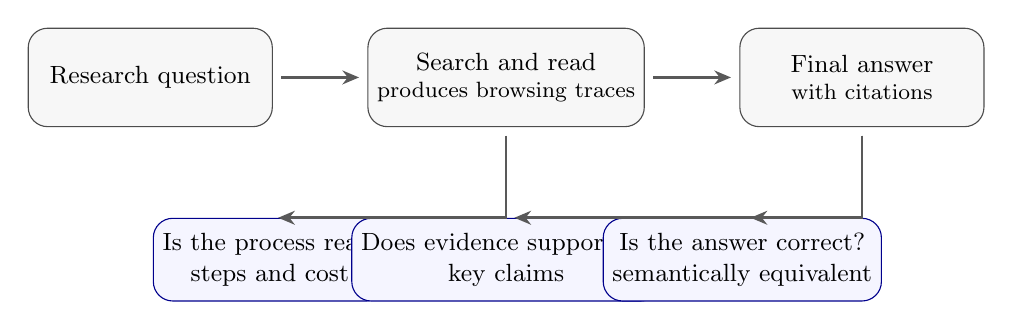
\begin{tikzpicture}[
  box/.style={draw=black!70,fill=black!3,rounded corners=7pt,minimum width=3.1cm,minimum height=1.25cm,align=center,font=\small},
  metric/.style={draw=blue!55!black,fill=blue!4,rounded corners=7pt,minimum width=2.9cm,minimum height=1.05cm,align=center,font=\small},
  arrow/.style={-{Stealth[length=6pt,width=5pt]},line width=1pt,black!65,shorten >=3pt,shorten <=3pt}
]
\node[box] (q) {Research question};
\node[box,right=1.2cm of q] (agent) {Search and read\\[-1pt]{\footnotesize produces browsing traces}};
\node[box,right=1.2cm of agent] (answer) {Final answer\\[-1pt]{\footnotesize with citations}};
\node[metric,below=1.15cm of agent,xshift=-3.0cm] (process) {Is the process real?\\steps and cost};
\node[metric,below=1.15cm of agent] (evidence) {Does evidence support it?\\key claims};
\node[metric,below=1.15cm of agent,xshift=3.0cm] (correct) {Is the answer correct?\\semantically equivalent};
\draw[arrow] (q) -- (agent);
\draw[arrow] (agent) -- (answer);
\draw[arrow] (agent.south) |- (process.north);
\draw[arrow] (answer.south) |- (evidence.north);
\draw[arrow] (answer.south) |- (correct.north);
\end{tikzpicture}
\end{document}
